\section{Performance Assessment}
%

The performance of the proposed method is assessed via comparison to that of a commercial software package considered to be among the state of the art. Performance is measured quantitatively for canonical image masks defined by spheres of various radii and locations and qualitatively for a variety of examples from real MRI and CT image scans. \\ \\
%
For the canonical cases, image masks are defined for each voxel ${v}$ by the following:
\begin{align} 
	v &=  \begin{cases}
		1, & \text{if}\ d \left(\bm{v_C},\bm{C}\right) <= R \\
		0, & \text{otherwise}
	\end{cases}
\end{align}
where $d$ is the Euclidean distance, $\bm{v_C}$ is the center of voxel $v$, $\bm{C}$ is the center of the spherical image mask, and $R$ is its radius. For these cases, the background image is assumed to have a 256 $\times$ 256 $\times$ 256 voxel resolution. \\ \\
%
In order to quantify performance, two error metrics are defined: shape error and volume error. These errors are defined in conjunction with a corresponding ``perfect sphere''. Every b-rep from these examples has an associated perfect sphere against which the error mismatch is measured. Built into these error metrics are two sources of error: the error of approximating the perfect sphere with a binary image mask, and the error of attempting to reconstruct the binary image mask with a b-rep. We will assume that the \textit{image-based accuracy}, as \cite{young_2008} refer to it, is negligible and focus on the ability of the method to ``converge to geometry''.\\ \\
%
The shape error measures the surface deviation of the resultant b-rep from the perfect sphere it is attempting to reconstruct. Each facet of the resulting b-rep is projected onto the underlying sphere. The normal of each facet is compared to the normal of the underlying sphere at the centroid of the projected facet via the magnitude of their cross product. A weighted sum is performed to integrate the area over the entire b-rep, and finally the sum is normalized by the surface area of the b-rep to provide a range of values of $\left[0,1\right]$. Thus, the shape error $e_s$ is defined as:
\begin{equation} 
	e_s = \frac{1}{A} \sum \limits_{f\in\mathcal{F}} \lVert {\bf n}_f \times {\bf n}_s \rVert
\end{equation}
where $A$ is the surface area of the b-rep, $f$ is a facet on the b-rep belonging to the set of all b-rep facets $\mathcal{F}$, ${\bm n}_f$ is the normal of facet $f$, and ${\bm n}_s$ is the normal of the associated sphere at the centroid of the projected facet $f$ onto the sphere. \\ \\
%
The volume error measures the unsigned difference in volume between the b-rep and associated perfect sphere it is meant to reconstruct. If we define the facet surface of facet $f$ as $\gamma_f$,  ${\bm x} \in \gamma_f$, $r = \lVert {\bm x} \rVert$, $d\alpha$ as an area element on the sphere of the projected b-rep facet, and again $R$ as the radius of the underlying perfect sphere, we define a normalized volume error $e_v$ as:
\begin{equation}
	e_v = \frac{1}{4\pi R^2} \Big[\sum \limits_{f \in \mathcal{F}\textsl{}} \int \limits_{\gamma_f} (r - R)^2 d\alpha \Big]^{1/2}
\end{equation}
Each b-rep facet is projected onto the underlying perfect sphere. Integrals are performed numerically on the projected facet. Six quadrature points were found to provide sufficent accuracy. Finally the quantity is normalized by the surface area of the underlying perfect sphere. SHOULD WE GO INTO MORE DETAIL IN EXPLAINING SHAPE AND VOLUME ERRORS? 
\\ \\
%
The shape and volume errors are compared between the commercial software and the proposed method as three parameters are independently varied for the canonical sphere case: 1) resulting b-rep resolution, 2) the sphere radius, and 3) the sphere center. The purpose of these comparions is to show that the proposed method perfoms comparably to a respected option, rather than specifically pointing to the supreriority of one method over the other. Standard options are chosen in the commercial to yield the best results for that approach, namely selected "Binarise before smoothing" and performing 100 iterations of smart mask smoothing. \\ \\
%
\figref{graph1} shows the shape and volume errors for the two methods as the b-rep resolution is varied for a spherical mask centered in the image with a radius $R = 80$ voxels. See~\figref{demos1} for a visual comparison of the image mask and represetative b-reps from the commercial code and proposed method. Default parameters are used in the commercial code for b-rep for number of vertices  $n >= 2587$. For resolutions coarser than that, the "target maximum error" was increased to allow results with $n < 2587$. When comparing the shape error of the two approaches, the proposed method performs at least as well as the commercial option for very coarse meshes, and actually performs measurably better for a wide range of realistic values. The shape error of the proposed method slightly increases with resolution for extremely fine meshes, as the decimation tool pushes the final b-rep toward a shape error of about $3\%$ of the raw b-rep coming out of the Voronoi parition prior to smoothing or decimation. For the volume error, the proposed method performs better b-reps with resolution less than about 5000 vertices, and asymptotes to a comparable value toward which the commercial software converges.\\ \\
\begin{figure}[ht!]
	\centering
	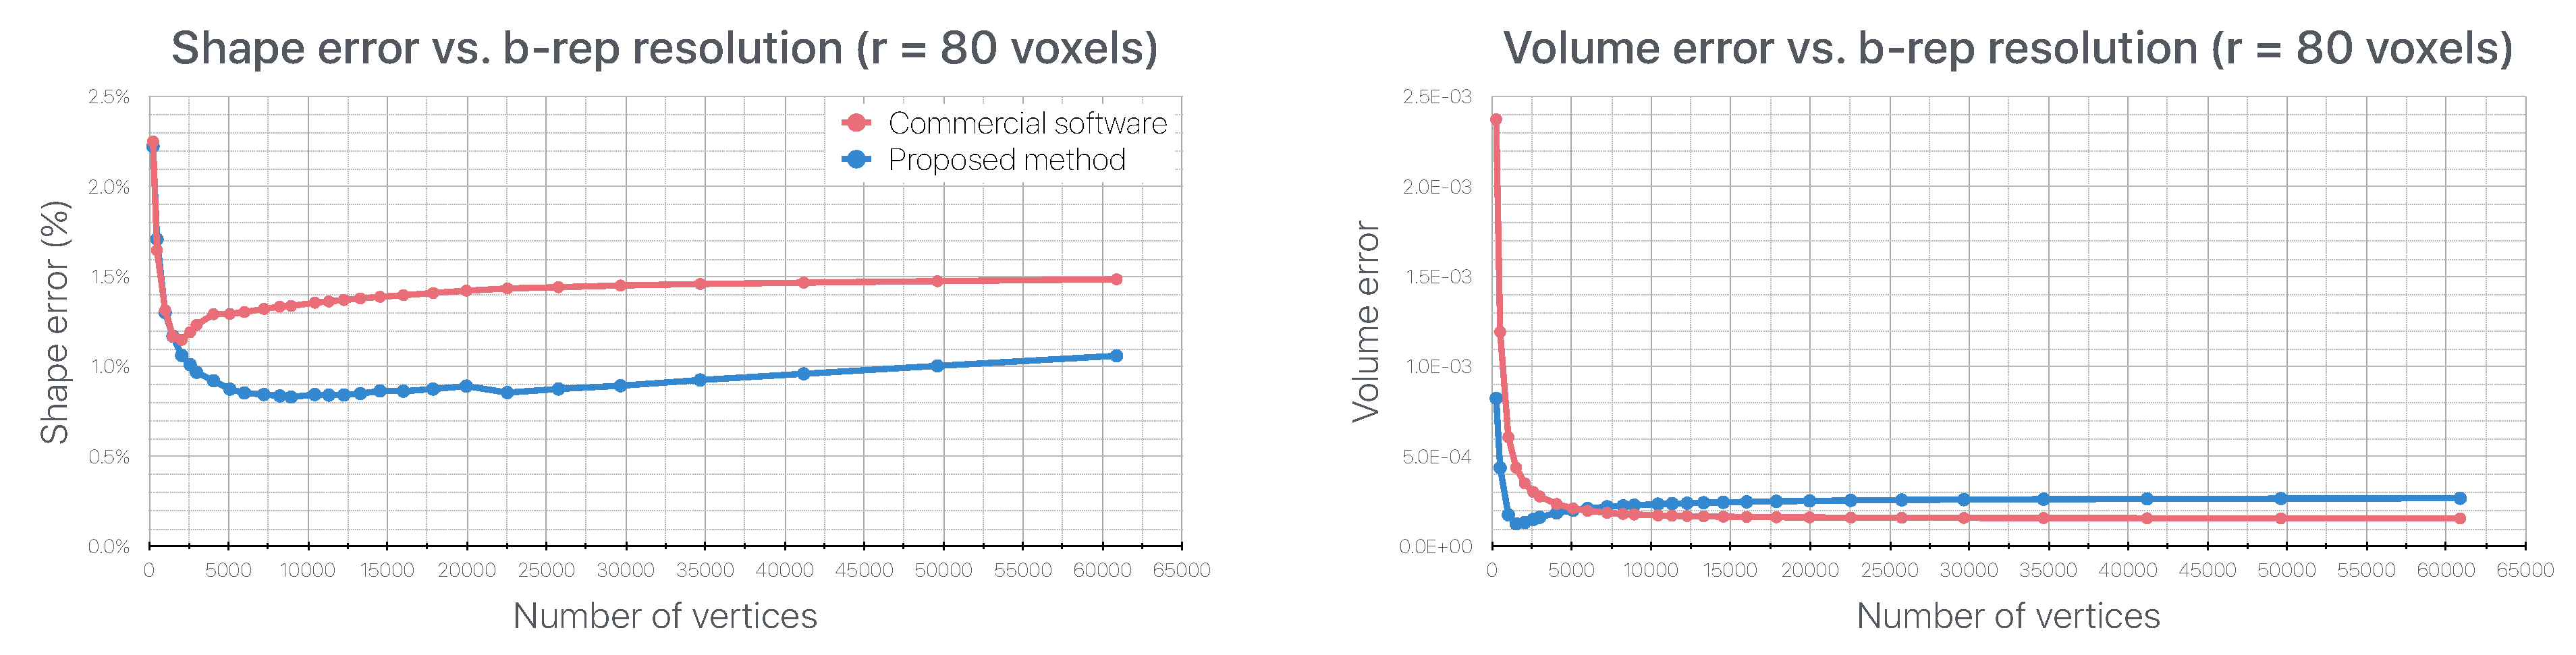
\includegraphics[scale=0.25]{media/7-performance/1-graph-1.pdf}
	\caption{Comparison of shape error (left) and volume error (right) between commercial software and proposed method as b-rep resolution is varied.}
	\label{fig:graph1}
\end{figure}
\begin{figure}[ht!]
	\centering
	\includegraphics[scale=0.25]{media/7-performance/3-demos-4.pdf}
	\caption{Image masks (green) and corresponding b-reps for commercial software (red) and proposed method (blue) for selected b-rep resolutions.}
	\label{fig:demos1}
\end{figure}
%
\figref{graph2}) shows the error metrics when the resulting b-rep resolution is kept fixed at $n = 10428$ vertices, while the radius of the spherical image mask if varied from 40 to 120 voxels. The spheres are once again always centered in the image. See~\figref{demos2} for representative examples of the image mask and resulting b-reps from the two methods. One can think of the sphere radius as an inverse measure of the curvature of the image mask. Larger radii correspond to smoother surfaces, whereas smaller radii correspond to regions of where surfaces are changing more rapidly. The proposed method has about a 2x faster convergence rate for both shape and volume erorrs compared to the commercial approach, albeit with larger coefficients in both cases. As expected, the proposed algorithm performs best for slowly-changing surfaces.
\begin{figure}[ht!]
	\centering
	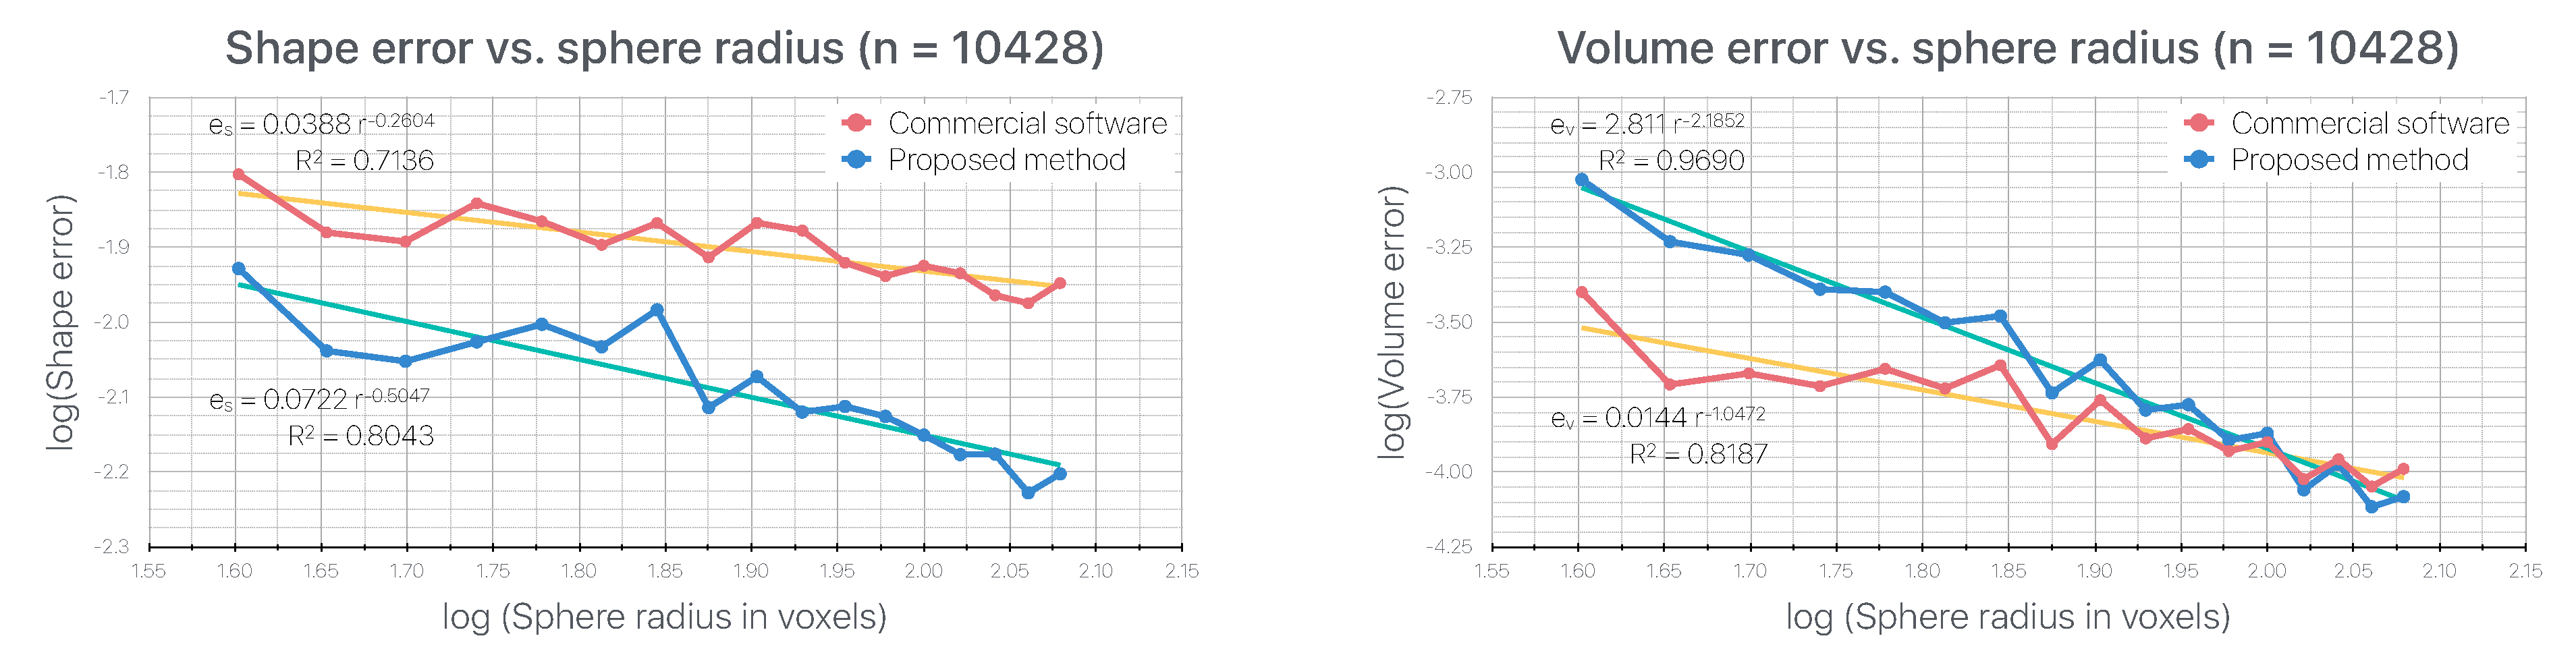
\includegraphics[scale=0.25]{media/7-performance/1-graph-2.pdf}
	\caption{Comparison of shape error (left) and volume error (right) between commercial software and proposed method as radius of sphere in image mask is varied.}
	\label{fig:graph2}
\end{figure}
\begin{figure}[ht!]
	\centering
	\includegraphics[scale=0.25]{media/7-performance/3-demos-5.pdf}
	\caption{Image masks (green) and corresponding b-reps for commercial software (red) and proposed method (blue) for selected sphere radii.}
	\label{fig:demos2}
\end{figure}
%
Finally, the two methods are compared for the cases where a sphere of $R = 80$ voxels is translated along a unit direction defined by the vector $\bm{i}  + 2\bm{j} + 3\bm{k}$. All resulting b-reps are tuned again to have a fixed resolution of n = 10428 vertices. The intent of this variation to test the sensitivity of the methods to the location of object within the image itself. Ideally the b-reps should be consistently accurate regardless of where the object is located, and indeed both methods show very low sensitivity to the translation of the object within the image, as shown in~\figref{graph3}. \\ \\
\begin{figure}[ht!]
	\centering
	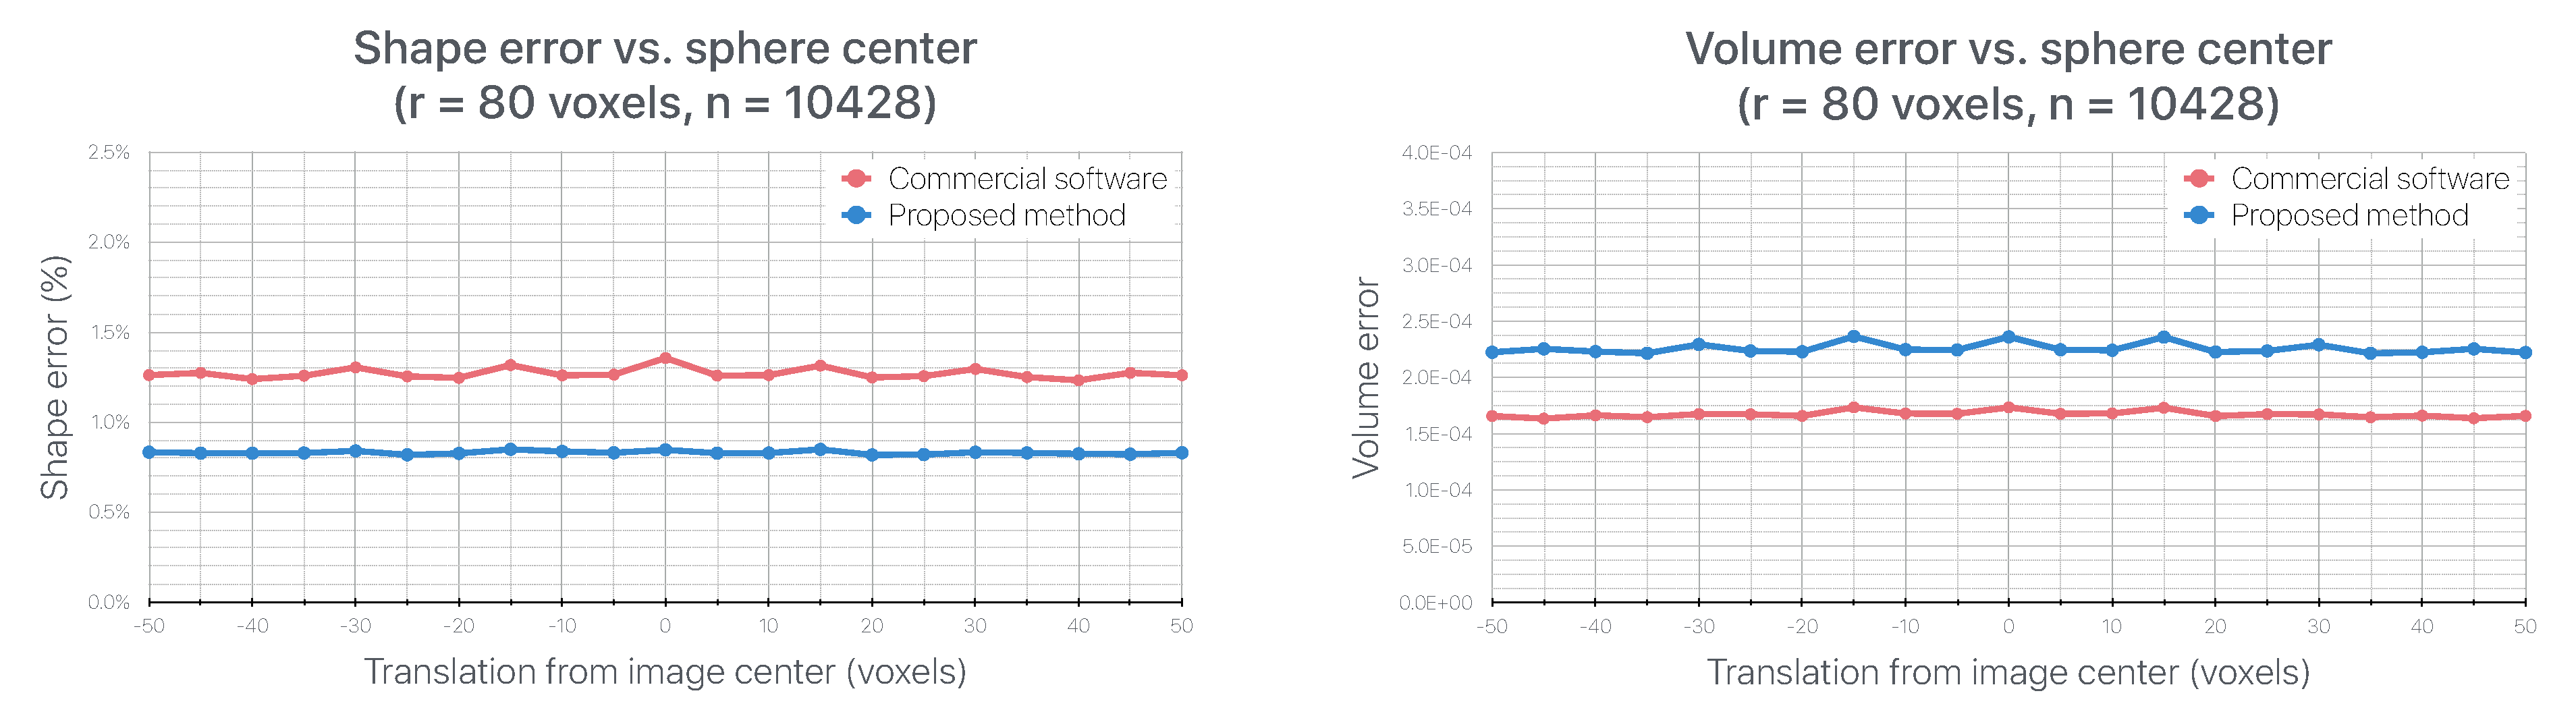
\includegraphics[scale=0.25]{media/7-performance/2-graph-3.pdf}
	\caption{Comparison of shape error (left) and volume error (right) between commercial software and proposed method as center of sphere in image mask is translated.}
	\label{fig:graph3}
\end{figure}
%
Qualitative comparisons are made for a number of real image examples). Images were segmented in Seg3D~\cite{Seg3D}. The resulting binary image masks were used as input to the two methods. B-rep resolutions were matched in all cases. See~\figref{example-meshes} for a comparison of image mask and resulting b-reps for a suite of examples. The proposed method perfoms comparably to the commercial approach in all cases, performing slighly better at smoothing surfaces and not quite as well for regions with high curvature. All examples completed for the proposed method on a 16 GB RAM laptop in less than 5 minutes.
\begin{figure}[ht!]
	\centering
	\includegraphics[scale=0.75]{media/7-performance/4-examples.pdf}
	\caption{Image masks (green) and corresponding b-reps for commercial software (red) and proposed method (blue) for various examples from MRI and CT. From top to botttom: brain~\cite{marcus_2007}, heart~\cite{winslow_2012}, lungs~\cite{rikxoort_2009}, distal femur~\cite{epperson_2013}, skull~\cite{clark_2013}, L5 lumbar~\cite{yao_2016}, pelvis~\cite{clark_2013}, upper left second molar (author's), liver~\cite{bilic_2019}, and example image with disjoint objects in image mask.}
	\label{fig:example-meshes}
\end{figure}